\subsection{Network to Learn Adaptive Step Sizes}
\label{section:Network to Learn Adaptive Step Size}
% \todo{add some commets;and refer this figure on network}
We propose to learn adaptive step sizes $\bm{\alpha}_t,\bm{\gamma}_t \in \mathbb{R}^d$ given the current iteration $t \in [1,L]$, where $L$ is the iteration number of the layer with unique parameters, and the initial token $\vx(0) \in \mathbb{R}^d$, using the network shown in Figure~\ref{fig:time embedding} and configurations in Table~\ref{tab:network to learn step sizes}.
\begin{figure}[htbp]
    \centering
    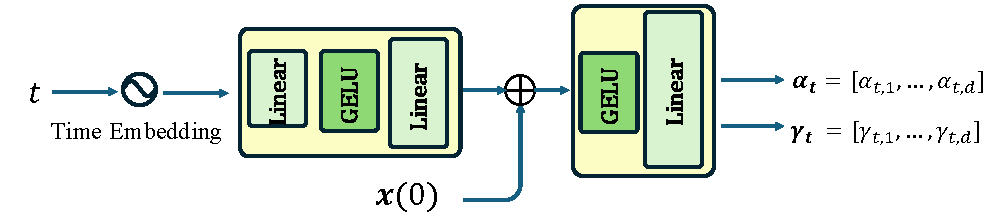
\includegraphics[width=\linewidth]{figures/time_embedding_v3.pdf}
        % \vskip -.2in
    \caption{Illustration of time embedding conditioned on the input to learn adaptive step size.}
    \label{fig:time embedding}
\end{figure}

\begin{table}[htbp]
\caption{Model configurations of network to learn adaptive step sizes.}
\label{tab:network to learn step sizes}
\centering
\begin{tabular}{ll}
        \toprule
        \textbf{Layer}  &  \textbf{Configuration} \\
        \midrule
        Time embedding  & 512 \\
        Linear & 512 $\times$ $d$ \\
        GELU & -- \\
        Linear & $d \times d$ \\
        GELU & -- \\
        Linear & $d \times 2d$ \\
        \bottomrule
\end{tabular}
\end{table}

% \begin{figure*}[htbp]
%   \centering
%   \begin{minipage}{0.7\textwidth}
%     \centering
%     \includegraphics[width=\linewidth]{time_embedding.pdf} % Replace with your image
%     \caption{Illustration of time embedding conditioned on the input to learn adaptive step size.}
%     \label{fig:time embedding}
%   \end{minipage}
%   \hfill
%   \begin{minipage}{0.28\textwidth}
%   \caption{Model configuration of network to learn adaptive step sizes.}
%   \label{tab:network to learn step sizes}
%     \centering
%     \resizebox{\linewidth}{!}{
%     \begin{tabular}{ll}
%         \toprule
%         Layer  &  Configurations \\
%         \midrule
%         Time embedding  & 512 \\
%         Linear & 512 $\times d$ \\
%         GELU & -- \\
%         Linear & $d \times d$ \\
%         GELU & -- \\
%         Linear & $d \times 2d$ \\
%         \bottomrule
%     \end{tabular}
%     }
%     \label{tab:sample}
%   \end{minipage}
% \end{figure*}

\subsection{Solving Sudoku}
\label{section:sudoku setup}
Solving a Sudoku puzzle requires filling a $9\times9$ board, with some digits (1-9) known and unknown entries marked as 0. The unknown entries must be filled with digits perfectly such that the board satisfies a certain rule, which can be seen as a logical reasoning task \citep{wang2019satnet}. We tackle this puzzle by predicting the digits to fill in, conditioned on the given digits. 
It can be viewed as a simplified masked modeling on synthetic data. Cross-entropy loss is computed exclusively on unknown entries. We train all models with 200 epochs, 16 batch size, AdamW \citep{loshchilov2018decoupled} with 0.1 weight decay, and learning rate from \num{1e-4} with cosine decay. The hidden dimension is set to 768. Tables~\ref{tab:training recipe for solving Sudoku} and~\ref{tab:model configuration for solving Sudoku} show the training recipe and model configurations for solving Sudoku. We train the model with 24 iterations and can evaluate beyond these iterations.

\begin{table*}[htbp]
    \centering
    \begin{minipage}[t]{0.49\textwidth}
    \centering
    \caption{Training recipe for solving Sudoku.}
    \label{tab:training recipe for solving Sudoku}
        % \resizebox{\linewidth}{!}{
        \begin{tabular}{ll}
        % \begin{tabularx}{\linewidth}{ll}
            \toprule
            \textbf{Hyperparameter}  & \textbf{Value} \\
            \midrule
            Epochs  &  200 \\
            Batch size & 16 \\
            $\#$ GPU & 1 $\times$ NVIDIA 3090 \\
            $\#$ Training samples & 9{,}000 \\
            $\#$ Evaluating samples & 1{,}000 \\
            Optimizer & AdamW \\
            $\beta_1, \beta_2$ & 0.9, 0.95 \\
            Weight decay & 0.1  \\
            Learning rate (lr) & \num{1e-4}\\
            LR decay & Cosine \\
            Gradient clipping & 1.0 \\
            \bottomrule
        % \end{tabularx}
        \end{tabular}
        % }
    \end{minipage}%
    \hfill
    \begin{minipage}[t]{0.49\textwidth}
    \centering
    \caption{Model configurations for solving Sudoku.}
    \vspace{-4pt}
    \label{tab:model configuration for solving Sudoku} 
        % \resizebox{\linewidth}{!}{
        \begin{tabular}{ll}
        % \begin{tabularx}{\linewidth}{ll}
            \toprule
            \textbf{Configuration}  & \textbf{Value} \\
            \midrule
            Vocabulary size & 10 \\
            Layer  &  1 \\
            Iterations $L$ & 24 \\
            Hidden dimension $d$ & 768 \\
            Feedforward ratio $M$ & $4d$ \\
            Number of heads $H$ & 12 \\
            Positional encoding & Learnable \\
            Time embedding condition & $\mX_0$ \\
            Time embedding frequency & 512 \\
            \midrule
            Total parameters & 5.20 M \\
            \bottomrule
        % \end{tabularx}
        \end{tabular}
        % }
    \end{minipage}
\end{table*}

\subsection{Image Classification}
\label{section:image classification setup}
Tables~\ref{tab:training recipe for image classfication} and~\ref{tab:model configuration for image classfication} present the training recipe and model configurations for image classification on CIFAR-10/100, while Tables~\ref{tab:training recipe for image classification im100} and~\ref{tab:model configuration for image classification im100} show those on ImageNet-100/1K. All models are trained with a learnable class token $[\texttt{CLS}]$. In practice, we use absolute sinusoidal positional encoding and adopt conditioning on $\mX_t$ for performance reasons. Table~\ref{tab:scaling modeling configuration} lists the configurations of different sizes, and it applies to other tasks as well.

% \begin{table}[htbp]
%     \centering
%     \begin{minipage}{0.45\textwidth}
%     \centering
%     \caption{Training Recipe for Image Classification.}
%     \label{tab:training recipe for image classfication}
%         \begin{tabular}{ll}
%             \toprule
%             Configuration  & Value \\
%             \midrule
%             Epochs  &  200 \\
%             Batch size & 128 (on 1 Nvidia 3090 GPU)\\
%             Number of training samples & 50k \\
%             Number of evaluating samples & 10k \\
%             Optimizer & Adam ($\beta_1=0.0,~\beta_2=0.95$)\\
%             Weight decay & 0.0  \\
%             Learning rate (lr) & 1e-4\\
%             Lr decay & Cosine \\
%             Gradient clipping & 1.0 \\
%             Input size & 224 \\
%             \bottomrule
%         \end{tabular}
        
%     \end{minipage}%
%     \hspace{0.08\textwidth} % Space between the tables
%     \begin{minipage}{0.45\textwidth}
%     \centering
%         \caption{Model Configuration for Image Classification $\texttt{Small}$).}
%     \label{tab:model configuration for image classfication}
        
%         \begin{tabular}{ll}
%             \toprule
%             Configuration  & Value \\
%             \midrule
%             Patch size & 16 \\
%             Layer  &  1 \\
%             Iterations & 12 \\
%             Hidden dimension $d$ & 384 \\
%             Feedforward ratio $M$ & $d$ \\
%             Number of heads $H$ & 6 \\
%             Positional encoding & Sinusoidal\\
%             Time embedding condition & $\mX_t$ \\
%             Time embedding frequency & 512 \\
%             \midrule
%             Number of parameters & 1.24 M \\
%             \bottomrule
%         \end{tabular}
%     \end{minipage}
% \end{table}
\begin{table*}[htbp]
    \centering
    \begin{minipage}[t]{0.49\textwidth}
        \centering
        \captionof{table}{Training recipe for image classification on CIFAR-10/100.}
        \label{tab:training recipe for image classfication}
        \begin{tabular}{ll}
        % \begin{tabularx}{\linewidth}{ll}
            \toprule
            \textbf{Hypersphere}  & \textbf{Value} \\
            \midrule
            Epochs  &  200 \\
            Batch size & 128 \\
            $\#$ GPU & 1 $\times$ NVIDIA 3090 \\
            $\#$ Training samples & 50{,}000 \\
            $\#$ Evaluating samples & 10{,}000 \\
            Optimizer & Adam \\
            $\beta_1, \beta_2$ & 0.9, 0.999 \\
            Weight decay & \num{5e-5}  \\
            Max learning rate (lr) & \num{1e-3}\\
            Min learning rate (lr) & \num{1e-5}\\
            LR decay & Cosine \\
            Warmup epochs & 5 \\
            Input size & 32 \\
            \bottomrule
        \end{tabular}
        % \end{tabularx}
    \end{minipage}%
    % \hspace{0.08\textwidth} % Space between the tables
    \hfill
    \begin{minipage}[t]{0.49\textwidth}
        \centering
        \captionof{table}{Model configurations ($\texttt{Small}$ Scaled-up) for image classification on CIFAR-10/100.}
        \label{tab:model configuration for image classfication}
        \begin{tabular}{ll}
        % \begin{tabularx}{\linewidth}{ll}
            \toprule
            \textbf{Configuration}  & \textbf{Value} \\
            \midrule
            Patch size & 8 \\
            Layer  &  1 \\
            Iterations $L$  & 12 \\
            Hidden dimension $d$ & 512 \\
            Feedforward ratio $M$ & $d$ \\
            Number of heads $H$ & 8 \\
            Positional encoding & Sinusoidal\\
            Time embedding condition & $\mX_t$ \\
            Time embedding frequency & 512 \\
            % \midrule
            % Number of parameters & 0.96 M \\
            \bottomrule
        \end{tabular}
        % \end{tabularx}
    \end{minipage}
\end{table*}


\begin{table*}[htbp]
    \centering
    \begin{minipage}[t]{0.49\textwidth}
        \centering
        \captionof{table}{Training recipe for image classification on ImageNet-100/1K.}
        \label{tab:training recipe for image classification im100}
        \begin{tabular}{ll}
        % \begin{tabularx}{\linewidth}{ll}
            \toprule
            \textbf{Hyperparameter}  & \textbf{Value} \\
            \midrule
            Epochs  &  200 \\
            Batch size & 256 \\
            $\#$ GPU & 1 $\times$ NVIDIA A100 \\
            $\#$ Training samples & 126{,}689/1{,}281{,}167 \\
            $\#$ Evaluating samples & 5{,}000/50{,}000 \\
            Optimizer & Adam \\
            $\beta_1, \beta_2$ & 0.9, 0.999 \\
            Weight decay & \num{5e-5}  \\
            Max learning rate (lr) & \num{1e-3}\\
            Min learning rate (lr) & \num{1e-5}\\
            LR decay & Cosine \\
            Warmup epochs & 5 \\
            Input size & 224 \\
            \bottomrule
        \end{tabular}
        % \end{tabularx}
    \end{minipage}%
    % \hspace{0.08\textwidth} % Space between the tables
    \hfill
    \begin{minipage}[t]{0.49\textwidth}
        \centering
        \captionof{table}{Model configurations ($\texttt{Small}$ Scaled-up) for image classification on ImageNet-100/1K.}
        \label{tab:model configuration for image classification im100}
        \begin{tabular}{ll}
        % \begin{tabularx}{\linewidth}{ll}
            \toprule
            \textbf{Configurations} & \textbf{Value} \\
            \midrule
            Patch size & 16 \\
            Layer  &  1 \\
            Iterations $L$ & 12 \\
            Hidden dimension $d$ & 512 \\
            Feedforward ratio $M$ & $d$ \\
            Number of heads $H$ & 8 \\
            Positional encoding & Sinusoidal\\
            Time embedding condition & $\mX_t$ \\
            Time embedding frequency & 512 \\
            % \midrule
            % Number of parameters & 1.21 M \\
            \bottomrule
        \end{tabular}
        % \end{tabularx}
    \end{minipage}
\end{table*}

\begin{table}[htbp]
\caption{Model configurations of different sizes.}
\label{tab:scaling modeling configuration}
\centering
\begin{tabular}{llll}
\toprule
\textbf{Configurations}  &  $\texttt{Small}$ & $\texttt{Small}$ Scale-up & $\texttt{Base}$\\
\midrule
Hidden dimension $d$  & 384 & 512 & 768 \\
Number of heads $H$  & 6 & 8 & 12 \\
\bottomrule
\end{tabular}

\end{table}


\subsection{Masked Image Modeling}
\label{section:masked image modeling setup}

We follow \citet{chang2022maskgit} using VQ-VAE to tokenize the images to $16\times16$ latent code with the codebook size of 1024 after resizing the input to $256\times256$. The masking ratio is randomly chosen between $[0,0.4]$, and the masked region is replaced by a learnable token. Training loss is computed only for the masked tokens. We also follow the iterative decoding process in \citet{chang2022maskgit} with $\text{temperature}=1$ and decoding step $T=24$. We also remove the MLP following the time embedding and set the embedding 
 frequency equal to the hidden dimension to save parameters, and we find out that this implementation works better. Tables~\ref{tab:training recipe for masked image modeling} and~\ref{tab:model configuration for masked image modeling} show the detailed training recipe and configurations.

We evaluate the quality of the reconstructed images of masking out $40\%$ of the images with $\texttt{Base}$ configurations. We report Peak Signal-to-Noise Ratio (PSNR), Structural Similarity Index Measure (SSIM) \citep{wang2004image}, Multi-Scale SSIM (MS-SSIM) \citep{wang2003multiscale}, Learned Perceptual Image Patch Similarity (LPIPS) \citep{zhang2018unreasonable} and Fr$\acute{\text{e}}$chet Inception Distance (FID) \citep{heusel2017gans} on the validation set (5k). 
\begin{table*}[htbp]
    \centering
    \begin{minipage}[t]{0.49\textwidth}
    \caption{Training recipe for masked image modeling.}
    \label{tab:training recipe for masked image modeling}
        \centering
        \begin{tabular}{ll}
        % \begin{tabularx}{\linewidth}{ll}
            \toprule
            \textbf{Hyperparameter}  & \textbf{Value} \\
            \midrule
            Epochs  &  300 \\
            Batch size & 256 ($64 \text{ per GPU} \times 4$)\\
            $\#$ GPU & 4 $\times$ NVIDIA A100 \\
            $\#$ Training samples & 126{,}689 \\
            $\#$ Evaluating samples & 5{,}000 \\
            Optimizer & AdamW \\
            $\beta_1, \beta_2$ & 0.9, 0.96 \\
            Weight decay & 0.1  \\
            Learning rate (lr) & \num{1e-4}\\
            LR decay & None \\
            Gradient clipping & 3.0 \\
            Input size & 256 \\
            \bottomrule
        \end{tabular}
        % \end{tabularx}
    \end{minipage}%
    % \hspace{0.08\textwidth} % Space between the tables
    \hfill
    \begin{minipage}[t]{0.49\textwidth}
        \caption{Model configurations for masked image modeling.}
    \label{tab:model configuration for masked image modeling}
        \centering
        \begin{tabular}{ll}
        % \begin{tabularx}{\linewidth}{ll}
            \toprule
            \textbf{Configuration}  & \textbf{Value} \\
            \midrule
            Vocabulary size & 1{,}025 \\
            Layer  &  1 \\
            Iterations & 12 \\
            Hidden dimension $d$ & 768 \\
            Feedforward ratio $M$ & $d$ \\
            Number of heads $H$ & 12 \\
            Positional encoding & Sinusoidal \\
            Time embedding condition & $\mX_0$ \\
            Time embedding frequency & 768 \\
            \midrule
            Total parameters & 3.94 M \\
            \bottomrule
        \end{tabular}
        % \end{tabularx}
    \end{minipage}
\end{table*}

\subsection{Definition of Effective Rank and Average Angle}
\label{section:definition}
We provide the formal definition of effective rank~\Eqref{eq:13} and average angle~\Eqref{eq:14} below. The effective rank is a continuous proxy of the full rank and, similar to the average angle, reflects the extent to which a set of vectors distributes uniformly. 
\begin{definition}[Effective Rank]
\label{definition:effective rank}
For a matrix $\mX \in \mathbb{R}^{d\times N}$, let $\Sigma=[\sigma_1,\dots,\sigma_r]$ be its singular values where $r$ is its full rank and denote $p_i = \sigma_i / \sum_{j=1}^r \sigma_j$ the discrete probability. The effective rank \citep{roy2007effective,guo2023contranorm} is defined as the exponential of the entropy 
\begin{equation}
\label{eq:13}
\exp(-\sum_{i=1}^r p_i \log p_i).
\end{equation}
\end{definition}

\begin{definition}[Average Angle]
\label{definition:average angle}
Given a set of vectors $\mX = [\vx_1, \dots, \vx_N] \in \mathbb{R}^{d\times N}$, the average angle of these vectors is 
\begin{equation}
\label{eq:14}
\operatorname{arccos} \frac{2}{N(N-1)}\sum_{i=1}^N\sum_{j=i+1}^{N}\frac{\vx_i^\top\vx_j}{\|\vx_i\|_2\|\vx_j\|_2}.
\end{equation}
\end{definition}

\subsection{Comparisons of Parameter Efficiency and Computational Cost}
\label{section:param and time}
\begin{table}[htbp]
\caption{Comparisons of parameters and computational cost of different architectures.}
\label{tab:comparisons of param and time}
\centering
\resizebox{0.95\linewidth}{!}{
\begin{tabular}{lllll}
\toprule
\textbf{Models} & \thead{\# Params (M)} & \thead{Memory (MB)} & \thead{GFLOPs} & \thead{Runtime (ms)} \\
\midrule
Transformer & 2.38  & 528  & 12.27	& $4.99_{\pm 0.14}$ \\
\textsc{CRATE}-T \citep{hu2024an} & 0.91  & 528  & 5.90 & $4.61_{\pm 0.17}$ \\
\textsc{CRATE} \citep{yu2023white} & 1.06  & 528  & 5.90 & $4.86_{\pm 0.19}$ \\
Energy Transformer \citep{hoover2024energy} & 1.50  & 670  & 6.19 & $21.95_{\pm 0.35}$ \\
\textsc{Hyper-SET} (Ours) & 1.55  & 528  & 6.81	& $8.03_{\pm 0.21}$\\ % \blue{$7.65_{\pm 0.20}$}
\bottomrule
\end{tabular}
}
\end{table}

\begin{table}[htbp]
\caption{Impact of step size and normalization strategies on computational cost and runtime. The configuration of our \textsc{Hyper-SET} is highlighted in \colorbox{gray!20}{gray}, which is designed to have $\operatorname{RMSNorm}$ placed after the subspace projection. Importantly, this configuration is not independent or disentangled but rather derived based on the proposed principled objective.}
\label{tab:bottleneck}
\centering
\resizebox{0.95\linewidth}{!}{
\begin{tabular}{l c c c c c}
\toprule
\thead{Step Size Strategy} & \thead{Pre-Norm} & \thead{LayerNorm} & \thead{\# Params (M)} & \thead{GFLOPs} & \thead{Runtime (ms)} \\
\midrule
\rowcolor{gray!20}
\cellcolor{white}\multirow{4}{*}{Learnable} & & & 1.55 & 6.81 & $8.03_{\pm 0.21}$ \\
 & \cmark & & 1.55 & 6.81 & $8.05_{\pm 0.22}$ \\
 & & \cmark & 1.55 & 6.84 & $7.31_{\pm 0.26}$ \\
 & \cmark & \cmark & 1.55 & 6.82 & $7.21_{\pm 0.28}$ \\
\midrule
\multirow{4}{*}{Fixed} & & & 0.91 & 4.98 & $5.70_{\pm 0.15}$ \\
 & \cmark & & 0.91 & 4.98 & $5.53_{\pm 0.25}$ \\
 & & \cmark & 0.91 & 5.01 & $4.86_{\pm 0.21}$ \\
 & \cmark & \cmark & 0.91 & 5.00 & $4.74_{\pm 0.18}$ \\
\bottomrule
\end{tabular}
}
\end{table}
To show the differences in parameters and computational cost incurred only by distinct architectures, we provide comparisons under the same width $d=384$. 
Empirically, we compare FLOPs and runtime in one forward pass using \href{https://github.com/MrYxJ/calculate-flops.pytorch}{\texttt{calflops}}, measured on a single NVIDIA A100 GPU, of our model and other baselines with a $3\times224\times224$ random input. Table~\ref{tab:comparisons of param and time} reports the results with mean and standard deviations averaged over 1{,}000 runs for robust measurements. Our model has fewer FLOPs as it has inherent structures like weight sharing due to mathematical design. 

To better understand the runtime performance of our model, we break down the contribution of key components in Table~\ref{tab:bottleneck}. The results reveal that the primary bottleneck in execution time stems largely from the facts that:
\begin{itemize}[leftmargin=*]
    \item We use an additional network to learn step sizes instead of keeping them fixed ($\sim$ 2.33\,ms);
    % \item we derive QK-Norm instead of the widely used Pre-Norm in self-attention ($\sim$ \blue{1.37\,ms}),
    \item The current default implementation of \texttt{torch.nn.RMSNorm()}, which we use to meet the hyperspherical constraints, is slower than \texttt{torch.nn.LayerNorm()} ($\sim$ 0.72\,ms).
\end{itemize}
% According to the above ablation, using pre-norm, layer-norm, fixed step sizes will roughly save 1.66ms, 2.05ms, 3.25ms, respectively. But this will deviate from our principled design and potentially lead to worse performance.

Currently, we trade some efficiency to allow for strong performance while keeping the principled design as transparent as possible with the additional modulation network for learned step sizes, which is adopted only for performance reasons rather than being a theoretically necessary component in our framework. In fact, our ablations that remove this extra network and fix the step sizes give similar runtime (5.70\,ms in Table~\ref{tab:bottleneck}), but the performance decreases greatly (81.45 on CIFAR-10 and 58.29 on CIFAR-100 in Table~\ref{tab:alternative design}). So, we believe there is still room for improvement in optimizing the step sizes schedule and further enhancing this minimalist implementation in future work.
%Currently, we trade some efficiency to allow for strong performance while keeping the principled design as transparent as possible. This trade-off may require studying the interaction between design objective and its optimization or applying/designing a more complex optimizer beyond gradient descent to further reduce the heuristics in the step sizes, which are now underexplored.

% We acknowledge this extra computational cost as one of our limitation in Appendix H.3, largely due to the modulation network that learns the step sizes (~2.33ms) which is adopted only for performance reasons rather than being a theoretically necessary component in our framework. It comes inevitably with some expenses to match Transformer with "white-box" design: more parameters (CRATE [1]) or more runtime cost (ours). In fact, we have provided ablations that remove this extra network and fix the step sizes, which gives similar runtime (5.70ms in Table 17), but the performance decreases greatly (81.45 on CIFAR-10 and 51.29 on CIFAR-100 in Table 4). So, we believe there is still room for improvement in optimizing the step sizes schedule and further enhancing this minimalist implementation in future work.

% \begin{table}[htbp]
% \caption{Bottleneck in runtime.}
% \label{tab:bottleneck}
% \centering
% \resizebox{0.8\linewidth}{!}{
% \begin{tabular}{llll}
% \toprule
% Models & $\#$ Params & GFLOPs & Runtime (ms) \\
% \midrule
% Ours & 1.55 M & 6.81	& $8.03_{\pm 0.21}$\\
% Ours (Pre-Norm)	&1.55 M	&6.81 &	$8.05_{\pm 0.22}$ \\ %\blue{$7.45_{\pm 0.21}$}
% Ours (LayerNorm) &1.55 M &6.84 & $7.31_{\pm 0.26}$ \\ %\blue{$7.02_{\pm 0.20}$}
% Ours (fixed step sizes)	&0.91 M	&4.98	& $5.70_{\pm 0.15}$ \\ % \blue{$5.04_{\pm 0.25}$}
% Ours (Pre-Norm \& LayerNorm) &	1.55 M &	6.82 & $7.21_{\pm 0.28}$ \\ % \blue{$7.10_{\pm 0.23}$}
% Ours (fixed step sizes \& Pre-Norm)	& 0.91 M & 4.98 & $5.53_{\pm 0.25}$ \\ % \blue{$5.02_{\pm 0.19}$}
% Ours (fixed step sizes \& LayerNorm) & 0.91 M & 5.01 & $4.86_{\pm 0.21}$ \\ % \blue{$4.57_{\pm 0.19}$}
% Ours (fixed step sizes \& Pre-Norm \& LayerNorm) &	0.91 M & 5.00 & $4.74_{\pm 0.18}$ \\ %\blue{$4.59_{\pm 0.23}$}
% \bottomrule
% \end{tabular}
% }
% \end{table}
